\documentclass[aspectratio=169,11pt]{beamer}

\usetheme{Madrid}

\usefonttheme{serif}

\usepackage{fontspec}

\setmainfont{Times New Roman}

\setsansfont{Arial}

\setmonofont{Menlo}

\usepackage{amsmath,amssymb,graphicx,tabularx}

\usepackage{hyperref}

\providecommand{\tightlist}{\setlength{\itemsep}{0pt}\setlength{\parskip}{0pt}}

\definecolor{SeminarRed}{HTML}{CC0100}

\setbeamercolor{normal text}{fg=black,bg=white}

\setbeamercolor{structure}{fg=SeminarRed}

\setbeamercolor{frametitle}{fg=black,bg=white}

\setbeamercolor{title}{fg=SeminarRed,bg=white}

\setbeamercolor{palette primary}{fg=white,bg=SeminarRed}

\setbeamercolor{palette secondary}{fg=white,bg=black}

\setbeamercolor{palette tertiary}{fg=white,bg=SeminarRed}

\setbeamercolor{palette quaternary}{fg=white,bg=black}

\setbeamercolor{block title}{fg=white,bg=SeminarRed}

\setbeamercolor{block body}{fg=black,bg=white}

\setbeamercolor{section in toc}{fg=black}

\setbeamercolor{itemize item}{fg=SeminarRed}

\setbeamercolor{enumerate item}{fg=SeminarRed}

\setbeamertemplate{navigation symbols}{}

\setbeamertemplate{footline}[frame number]

\setbeamercolor{page number in head/foot}{fg=black,bg=white}

\setbeamertemplate{frametitle continuation}{}

\setbeamersize{text margin left=0.7cm,text margin right=0.7cm}

\hypersetup{colorlinks=true,urlcolor=SeminarRed,linkcolor=SeminarRed}

\AtBeginSection[]{\begin{frame}[plain]\vfill\centering\LARGE\color{SeminarRed}\insertsectionhead\vfill\end{frame}}

\title{Seminário Modelagem Econômica Baseada em Agentes - SCX5013}

\date{}

\begin{document}

\begin{frame}[plain]\vfill\centering{\Huge\bfseries\color{SeminarRed} Seminário Modelagem Econômica Baseada em Agentes - SCX5013}\vspace{0.8cm}\par{\color{black}\rule{0.55\textwidth}{0.8pt}}\vspace{0.5cm}\par{\color{black} Daniel Andrade - Outubro, 2026}\vfill\end{frame}

\section{1. Visão geral e motivação do modelo}

\begin{frame}[allowframebreaks]{1.1 Trabalhos abordados}
\normalsize
Iremos abordar o modelo proposto nos trabalhos:

\begin{itemize}
\item
  \texttt{Economic\ forecasting\ with\ an\ agent-based\ model}, Poledna et al.~(2023)
\item
  \texttt{BeforeIT.jl:\ High-Performance\ Agent-Based\ Macroeconomics\ Made\ Easy}, implementação open source na linguagem Julia por Glielmo et al.~(2025)
\end{itemize}

Utilizaremos a implementação em Julia para explorar o modelo de maneira prática. Julia é uma linguagem de programação que pretende ser ao mesmo tempo fácil de programar e rápida.
\end{frame}


\begin{frame}[allowframebreaks]{1.2 Motivadores do modelo}
\normalsize
As principais motivações do trabalho são:

\begin{itemize}
\item
  Realizar \texttt{previsões\ macroeconômicas} utilizando modelagem baseada em agentes.
\item
  Construir uma modelagem verossimilhante, calibrando o modelo de acordo com as estatísticas governamentais e executando a simulação com escala 1:1 da população do país.
\end{itemize}

O modelo inicial foi calibrado para a economia da Áustria, que é um país pequeno e altamente integrado com a economia externa (\(\approx 9M\) habitantes e \(\approx 50\%\) do PIB em importações/exportações).

O trabalho se encaixa nas características centrais dos modelos macroeconômicos baseados em agentes definidos pela revisão de Dawid e Delli Gatti (2018):
\end{frame}


\begin{frame}[allowframebreaks]{1.2 Motivadores do modelo}
\normalsize
\begin{quote}
``Em modelos macroeconômicos baseados em agentes, tipos diferentes de agentes heterogêneos com regras comportamentais e de expectativas interagem através de protocolos de mercado explícitos e variáveis meso e macroeconômicas são determinadas através da agregação dos resultados dessa população de agentes.'' (tradução livre)
\end{quote}
\end{frame}


\begin{frame}[allowframebreaks]{1.3 Inicialização do modelo}
\normalsize
Com os comandos abaixo inicializamos as condições de partida do modelo:

\begin{itemize}
\item
  Parâmetros (fixos).
\item
  Variáveis de estado (evoluem no tempo).
\end{itemize}
\end{frame}


\begin{frame}[allowframebreaks]{1.4 Agentes do modelo}
\normalsize
Podemos inspecionar as condições iniciais para nos informarmos sobre os agentes do modelo.
\end{frame}


\begin{frame}{1.4 Agentes do modelo}
\small
\begin{tabularx}{\textwidth}{lXX}
Row & Agent type & Count \\
\hline
1 & Trabalhadores ativos (empregados e desempregados) & 4743.0 \\
2 & Trabalhadores inativos & 4130.0 \\
3 & Empresas (e donos de empresas) & 624.0 \\
4 & Governos (central e locais) & 156.0 \\
5 & Consumidores externos & 312.0 \\
6 & Empresas estrangeiras (importadoras) & 62.0 \\
7 & Banco central (Taxa Básica) & 0.16 \\
8 & Banco comercial representativo (Taxa de Juros) & 2.84 \\
\end{tabularx}
\end{frame}


\begin{frame}[allowframebreaks]{1.5 Resultados do modelo na prática}
\normalsize
Vamos explorar os resultados do modelo na prática.

Cada passo equivale a 47 funções executadas sequencialmente. Verificamos então como as estatísticas agregadas da economia evoluem ao longo do tempo:

\begin{itemize}
\item
  Crescimento da economia
\item
  Inflação
\item
  Desemprego
\end{itemize}

Observamos também que o modelo possui propriedades emergentes que também são verificadas na economia, como:

\begin{itemize}
\item
  Oscilações econômicas
\item
  Tendência de crescimento sustentada do PIB (países industrializados)
\end{itemize}
\end{frame}


\begin{frame}{1.5 Resultados do modelo na prática}
\centering
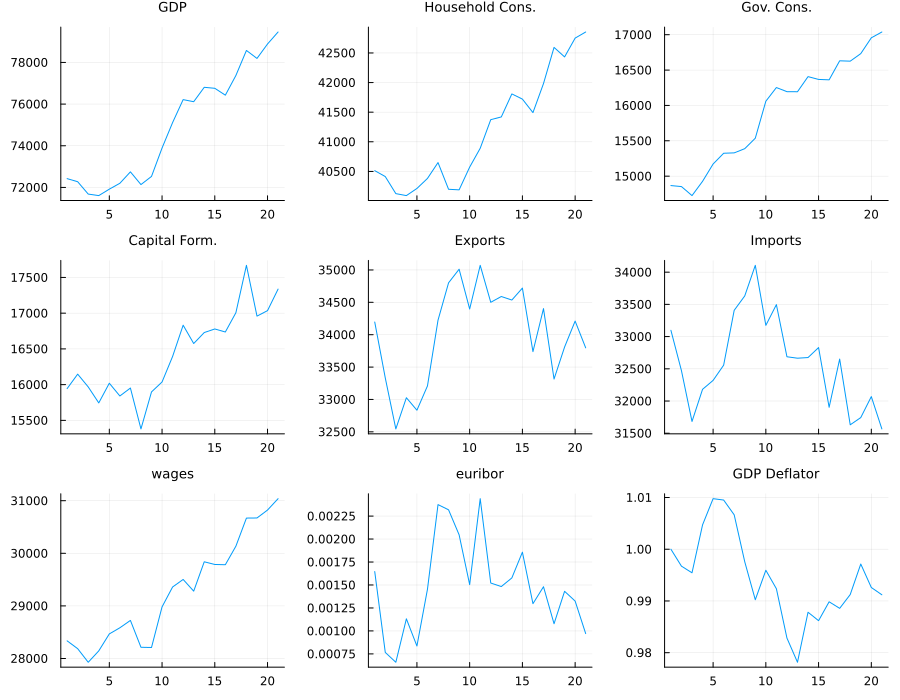
\includegraphics[width=0.95\textwidth,height=0.78\textheight,keepaspectratio]{assets/celula-16.png}
\end{frame}


\begin{frame}[allowframebreaks]{1.6 Regras de evolução temporal}
\normalsize
Cada etapa temporal do modelo equivale a um \texttt{trimestre}. As etapas-chave que levam o modelo de \(t\) para \(t+1\) são:

\begin{description}
\item[1.] Formação de expectativas coletivas - regra AR(1) 

\item[2.] Execução dos choques exógenos - regra AR(1)

\item[3.] Execução dos mercados de crédito e trabalho

\item[4.] Execução dos mercados de bens  

\item[4.] Atualização da contabilidade
\end{description}
\end{frame}


\begin{frame}{1.6 Regras de evolução temporal}
\centering
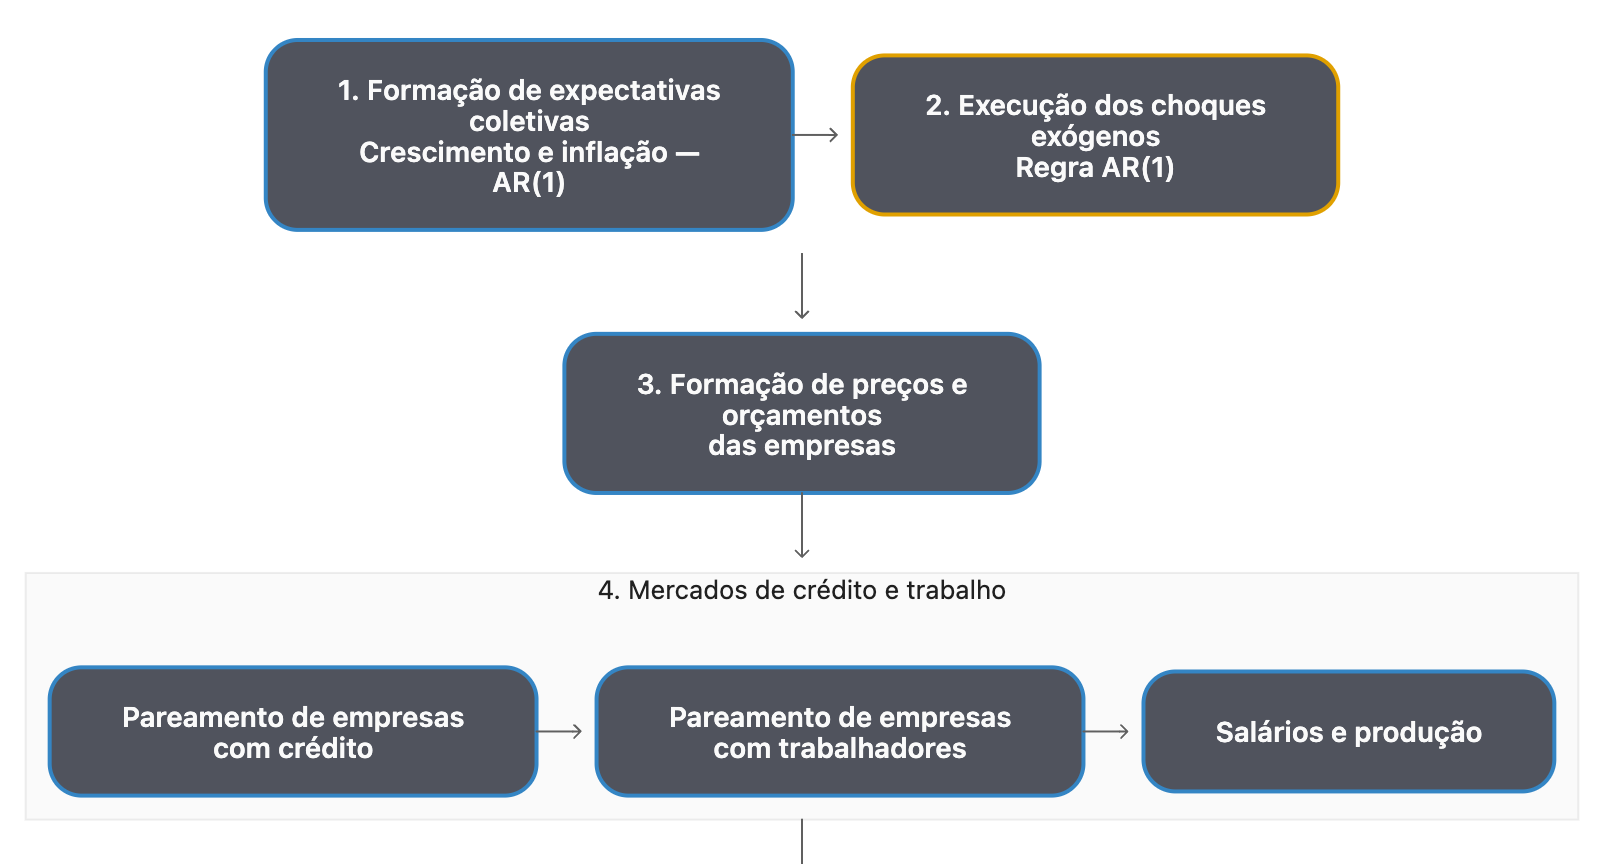
\includegraphics[width=0.95\textwidth,height=0.78\textheight,keepaspectratio]{assets/celula-19-novo-fluxo-completo-mermaid-diagram-parte-1.png}
\end{frame}


\begin{frame}{1.6 Regras de evolução temporal}
\centering
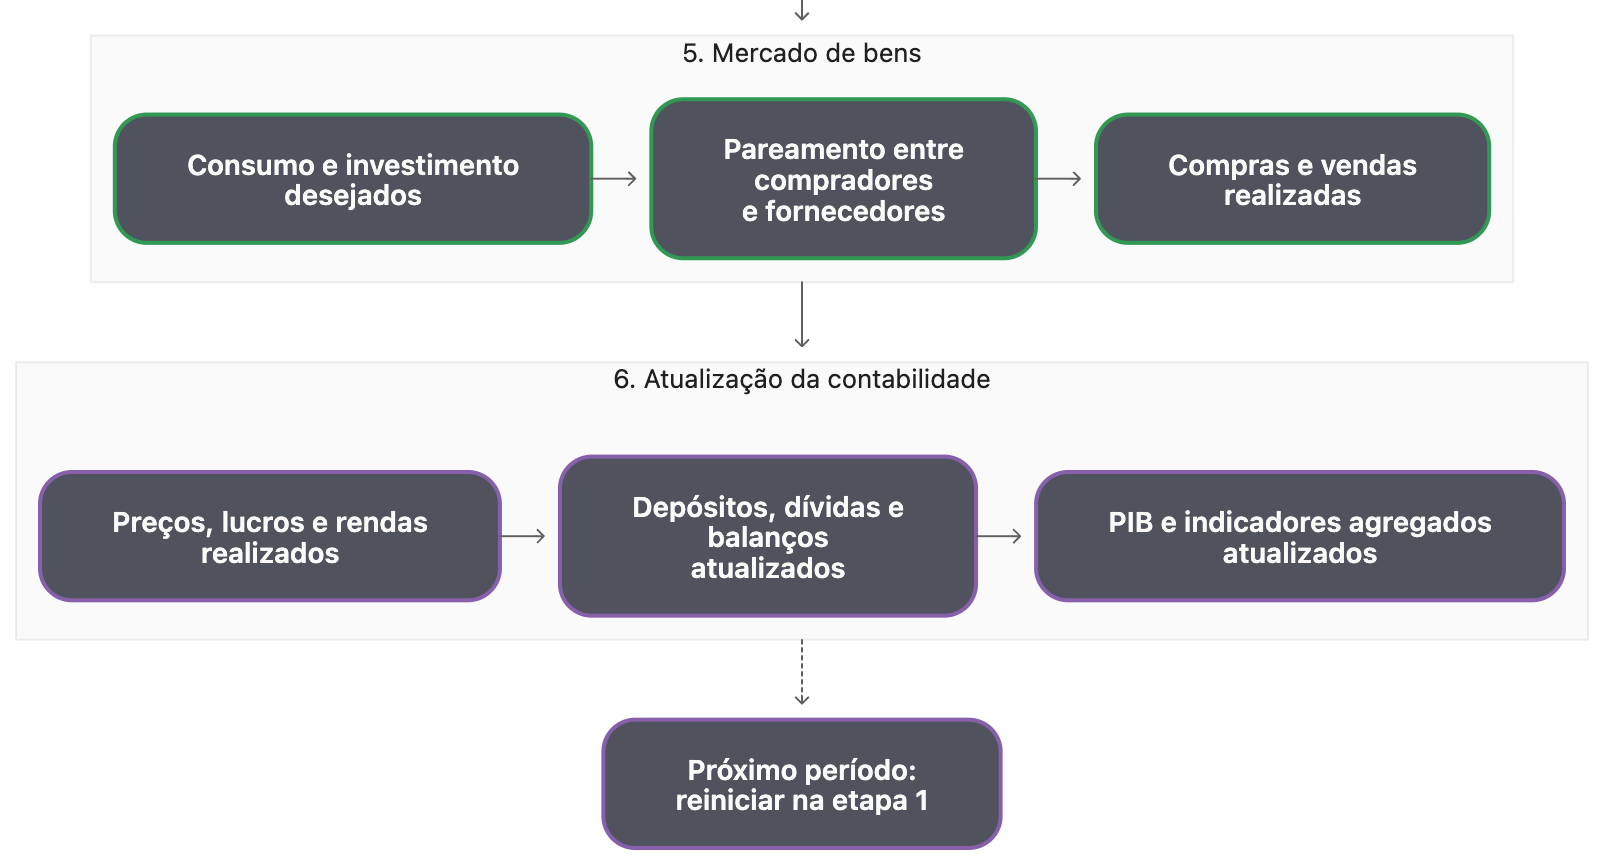
\includegraphics[width=0.95\textwidth,height=0.78\textheight,keepaspectratio]{assets/celula-19-novo-fluxo-completo-mermaid-diagram-parte-2.png}
\end{frame}


\section{2. Regras autoregressivas de ordem 1 - AR(1)}

\begin{frame}[allowframebreaks]{2.1 O que são as relações AR(1)}
\normalsize
As regras autoregressivas de ordem 1 são o cálculo de uma variável no futuro, \(z_{t}\), a partir de uma relação linear desta variável no passo de tempo anterior e uma inovação/choque de variância finita \(\epsilon_{t}\), ou seja:

\[y_{t} = a + \rho y_{t-1} + \epsilon_{t} 
\qquad 0 \leq \rho < 1\]

Em Poledna et al., essa regra é utilizada para:

\begin{itemize}
\item
  Formação das expectativas coletivas de crescimento do PIB e inflação.
\item
  Modelagem de eventos exógenos com choques aleatórios (importações, exportações, gasto do governo, inflação e crescimento da área do euro).
\end{itemize}
\end{frame}


\begin{frame}[allowframebreaks]{2.2 Uso nas expectativas}
\normalsize
Com relação às expectativas de PIB e inflação:

\begin{itemize}
\item
  A cada semestre os agentes calculam os parâmetros de maneira otimizada (com o melhor fit possível com relação aos dados históricos).
\item
  Na prática, os agentes estão aprendendo e atualizando suas expectativas, o que os torna \texttt{adaptativos}.
\end{itemize}

Por exemplo, para as empresas a produção desejada no próximo período é:

\[
Q_i^s=Q_i^d(1+\gamma^e)
\]

\[
\begin{aligned}
i &: \text{empresa considerada}\\
Q_i^s &: \text{produção desejada pela empresa }i\\
Q_i^d &: \text{demanda pelo produto da empresa }i\text{ no período anterior}\\
\gamma^e &: \text{taxa esperada de crescimento da economia}
\end{aligned}
\]

Para os consumidores o consumo desejado no próximo período é:

\[
Y_h^e=
\left[w_h(1-\tau_{\mathrm{SIW}})(1-\tau_{\mathrm{INC}})+sb^{\mathrm{other}}\right]
\bar P_{HH}(1+\pi^e)
\]
\end{frame}


\begin{frame}[allowframebreaks]{2.2 Uso nas expectativas}
\normalsize
\[
\begin{aligned}
Y_h^e &: \text{renda disponível esperada do trabalhador }h\\
w_h &: \text{salário antes dos descontos}\\
\tau_{\mathrm{SIW}} &: \text{contribuição social do trabalhador}\\
\tau_{\mathrm{INC}} &: \text{imposto de renda}\\
sb^{\mathrm{other}} &: \text{outros benefícios sociais}\\
\bar P_{HH} &: \text{índice de preços do consumo das famílias}\\
\pi^e &: \text{inflação esperada}
\end{aligned}
\]

Abaixo vamos ilustrar como as regras AR(1) são calculadas na prática.
\end{frame}


\begin{frame}{2.2 Uso nas expectativas}
\centering
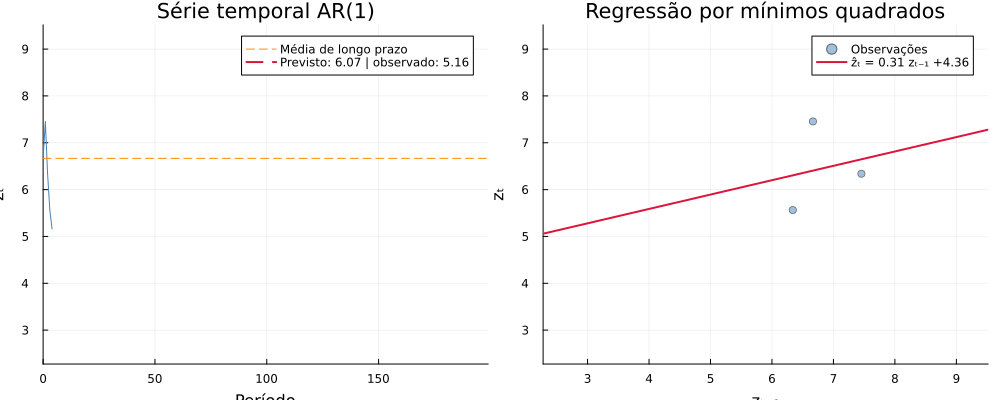
\includegraphics[width=0.95\textwidth,height=0.78\textheight,keepaspectratio]{assets/celula-25-quadro-000.png}
\end{frame}


\begin{frame}{2.2 Uso nas expectativas}
\centering
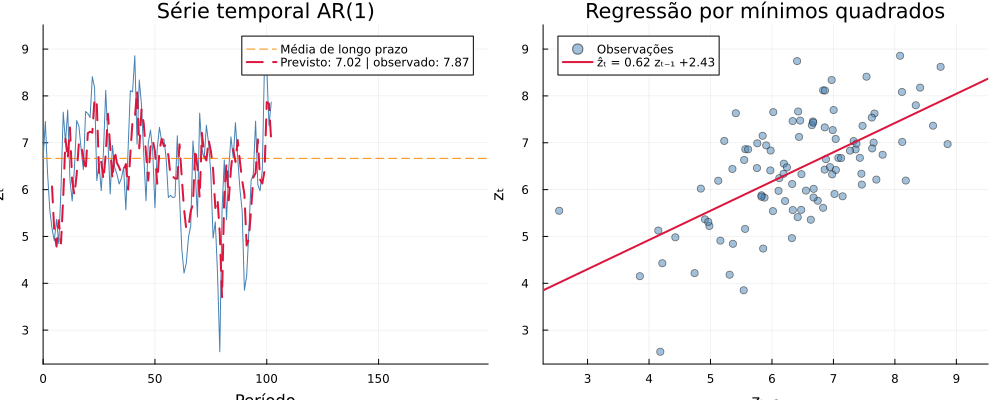
\includegraphics[width=0.95\textwidth,height=0.78\textheight,keepaspectratio]{assets/celula-25-quadro-098.png}
\end{frame}


\begin{frame}{2.2 Uso nas expectativas}
\centering
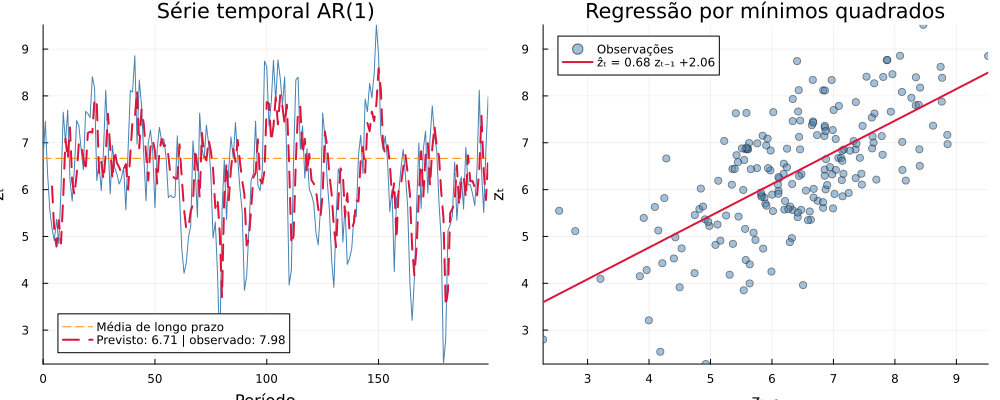
\includegraphics[width=0.95\textwidth,height=0.78\textheight,keepaspectratio]{assets/celula-25-quadro-195.png}
\end{frame}


\begin{frame}[allowframebreaks]{2.2 Uso nas expectativas}
\normalsize
Os argumentos principais para o uso dessa regra são:

\begin{itemize}
\item
  É uma regra simples mas poderosa, onde os agentes ignoram as não linearidades que estão por trás das variáveis econômicas mas conseguem construir uma previsão da direção da econômia que instrumenta suas decisões.
\item
  Os autores indicam que regras como esta já foram verificadas experimentalmente para comportamento humano com relação à previsão de variáveis econômicas.
\item
  Os dados utilizados para o cálculo das regressões são os dados reais da economia austríaca o que reforça a verossimilhança do modelo.
\end{itemize}
\end{frame}


\begin{frame}[allowframebreaks]{2.2 Uso nas expectativas}
\normalsize
No longo prazo, o aprendizado pode aproximar o sistema de um \texttt{Behavioural\ Learning\ Equilibrium\ (BLE)}, uma situação em que a média e a autocorrelação de primeira ordem dos agentes coincidem com as observadas na economia gerada pelo modelo, como demonstrado em (Hommes e Zhu, 2014).

Assim, o modelo busca capturar a tendência de crescimento sustentado verificado nos países industrializados.
\end{frame}


\begin{frame}{2.2 Uso nas expectativas}
\centering
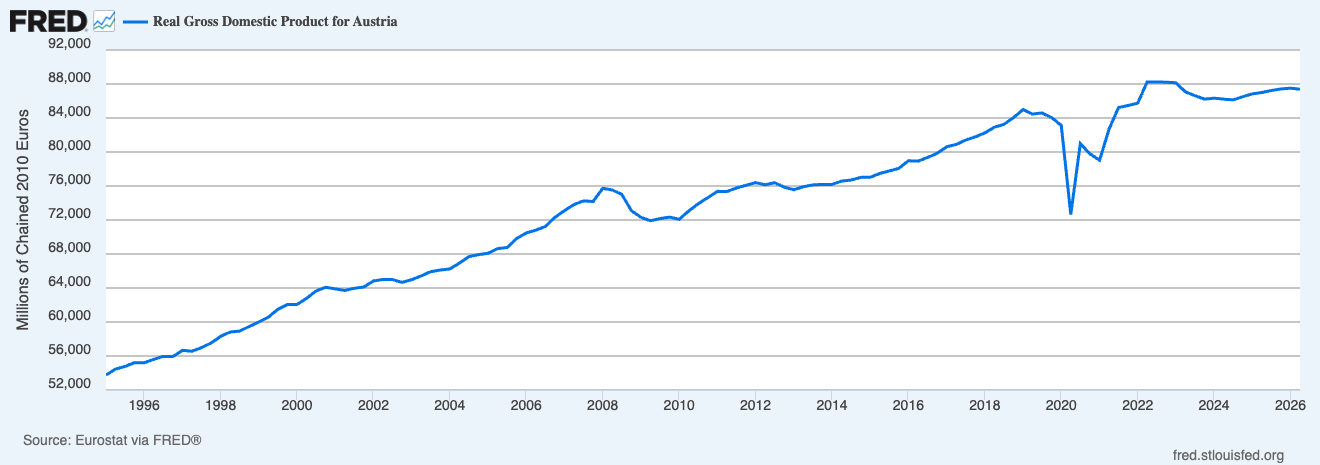
\includegraphics[width=0.95\textwidth,height=0.78\textheight,keepaspectratio]{assets/fredgraph.png}
\end{frame}


\begin{frame}[allowframebreaks]{2.3 Uso nos choques exógenos}
\normalsize
O PIB da área do EURO é calculado através de um processo AR(1) que utiliza um choque exógeno retirado de uma distribuição normal:

\[
Y_{EA,t}=
\exp\left[
\alpha_{Y,EA}\log(Y_{EA,t-1})
+\beta_{Y,EA}
+\varepsilon_{Y,EA,t}
\right]
\]

\[
\begin{aligned}
Y_{EA,t} &: \text{valor da série }Y\text{ para }EA\text{ no período }t\\
Y_{EA,t-1} &: \text{valor da mesma série no período anterior}\\
\alpha_{Y,EA} &: \text{coeficiente de persistência da série}\\
\beta_{Y,EA} &: \text{termo constante na escala logarítmica}\\
\varepsilon_{Y,EA,t} &: \text{choque ou erro no período }t\\
EA &: \text{identificador da série ou grupo; significado depende do modelo}\\
t &: \text{período de tempo}
\end{aligned}
\]
\end{frame}


\section{3. Calibração para as contas nacionais}

\begin{frame}[allowframebreaks]{3.1 Estratégia de calibração}
\normalsize
O trabalho busca se adequar às estatísticas de contabilidade nacional.

Nesse sentido, os parâmetros do modelo são:

\begin{itemize}
\item
  Retirados diretamente das estatísticas oficiais.
\item
  Ou calculados a partir delas.
\end{itemize}

Isto torna o modelo mais verossimilhante e reduz a necessidade de estimação de parâmetros livres, uma das grandes críticas aos ABMs.

Abaixo iremos explorar alguns dos parâmetros/estatísticas mais interessantes do modelo.
\end{frame}


\begin{frame}[allowframebreaks]{3.1 Estratégia de calibração}
\small
\begin{description}
\item[Row] 1
\item[Parametro] H\_act
\item[Valor] 4743
\item[Significado] Agentes economicamente ativos
\item[Calculo] empregados + desempregados + proprietários de firmas + 1
\item[Fonte] Censo e demografia empresarial
\end{description}
\end{frame}


\begin{frame}[allowframebreaks]{3.1 Estratégia de calibração}
\small
\begin{description}
\item[Row] 2
\item[Parametro] tau\_INC
\item[Valor] 21.34\%
\item[Significado] Alíquota média de imposto de renda das famílias
\item[Calculo] (IR familiar + impostos de capital) / (salários + renda de propriedade + renda mista - contribuições sociais)
\item[Fonte] Estatísticas do governo e contas setoriais
\end{description}
\end{frame}


\begin{frame}[allowframebreaks]{3.1 Estratégia de calibração}
\small
\begin{description}
\item[Row] 3
\item[Parametro] psi
\item[Valor] 90.97\%
\item[Significado] Parcela da renda disponível destinada ao consumo
\item[Calculo] (consumo das famílias + impostos sobre consumo) / renda disponível
\item[Fonte] Tabelas de insumo-produto e contas setoriais
\end{description}
\end{frame}


\begin{frame}[allowframebreaks]{3.1 Estratégia de calibração}
\small
\begin{description}
\item[Row] 4
\item[Parametro] theta\_UB
\item[Valor] 35.86\%
\item[Significado] Reposição do benefício de desemprego sobre o salário bruto
\item[Calculo] 0,55 × (1 - tau\_INC) × (1 - tau\_SIW)
\item[Fonte] Regra austríaca: 55\% da renda líquida
\end{description}
\end{frame}


\begin{frame}[allowframebreaks]{3.2 Matriz insumo-produto}
\normalsize
A matriz insumo-produto, concebida inicialmente por Leontief, descreve as relações entre os diferentes setores produtivos:

\begin{itemize}
\item
  Cada linha representa um setor fornecedor \(s\) e cada coluna um setor produtor \(g\).
\item
  A entrada \(a_{sg}\) é a participação do setor \(s\) nos insumos intermediários usados pelo setor \(g\). Cada coluna soma 1.
\end{itemize}

Como exemplo, abaixo temos uma demonstração dos insumos do setor de educação.
\end{frame}


\begin{frame}{3.2 Matriz insumo-produto}
\centering
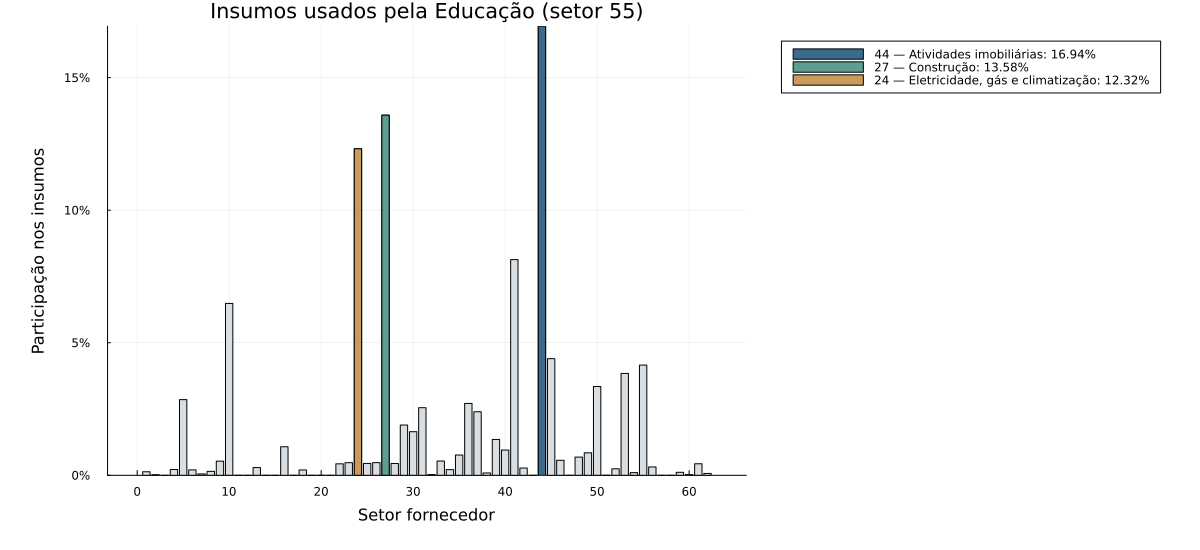
\includegraphics[width=0.95\textwidth,height=0.78\textheight,keepaspectratio]{assets/celula-37.png}
\end{frame}


\begin{frame}[allowframebreaks]{3.2 Matriz insumo-produto}
\normalsize
Abaixo, um mapa de calor da matriz de insumo-produto. Os pontos mais brilhantes são aqueles que representam maior relação entre setor e produto.
\end{frame}


\begin{frame}{3.2 Matriz insumo-produto}
\centering
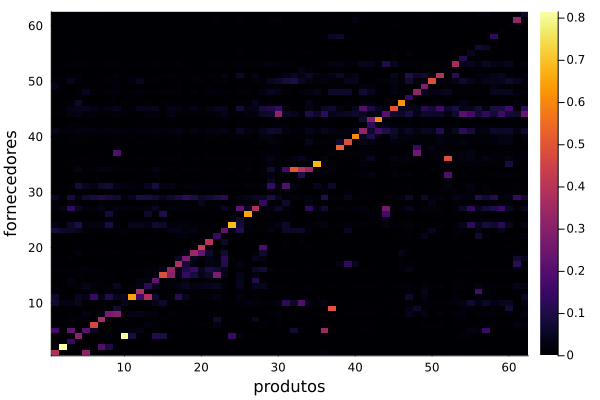
\includegraphics[width=0.95\textwidth,height=0.78\textheight,keepaspectratio]{assets/celula-39.png}
\end{frame}


\begin{frame}[allowframebreaks]{3.2 Matriz insumo-produto}
\normalsize
Em um texto de 1951 sobre a matriz insumo-produto, Leontief diz:

\begin{quote}
O efeito de um acontecimento num ponto em particular é transmitido ao resto da economia, passo a passo, mediante uma série de transações que vinculam a totalidade do sistema num só conjunto. Uma tabela de razões para o conjunto da economia nos dá, com tanto detalhe quanto quisermos, um quadro quantitativamente determinado da estrutura interna do sistema. Isso possibilita o cálculo detalhado das conseqüências decorrentes da introdução no sistema de variações sugeridas pelo problema teórico ou prático que enfrentamos.
\end{quote}

Nesse sentido, o modelo vai ao encontro da visão original da matriz ao propor a simulação dos acontecimentos econômicos a partir de relações verificadas empiricamente.
\end{frame}


\begin{frame}[allowframebreaks]{3.2 Matriz insumo-produto}
\normalsize
Além disso, ao falar do problema de inversão da matriz (saber os insumos necessários a partir do resultado desejado) , ele coloca:

\begin{quote}
Uma típica solução geral de uma tabela de 42 setores para 1939 demorou 56 horas no computador Mark II de Harvard.
\end{quote}

Hoje, isso pode ser feito em segundos. Para obter os coeficientes por unidade produzida, dividimos cada coluna de \(a_{sg}\) por \(\beta_g\), a razão entre produção e consumo intermediário do setor \(g\). A inversa de Leontief é então \((I-A)^{-1}\), com \(A_{sg}=a_{sg}/\beta_g\).
\end{frame}


\begin{frame}{3.2 Matriz insumo-produto}
\small
\begin{tabularx}{\textwidth}{lXX}
Row & setor & producao\_necessaria \\
\hline
1 & 55 & 1.00581 \\
2 & 24 & 0.0414947 \\
3 & 27 & 0.0302856 \\
4 & 44 & 0.0286633 \\
5 & 4 & 0.0178657 \\
6 & 41 & 0.0175113 \\
7 & 45 & 0.0150364 \\
8 & 10 & 0.0114625 \\
9 & 53 & 0.00859417 \\
10 & 50 & 0.00776177 \\
\end{tabularx}
\end{frame}


\begin{frame}[allowframebreaks]{3.3 Consistência fluxo-estoque}
\normalsize
Outro ponto importante é a consistência estoque-fluxo do modelo:

\begin{itemize}
\item
  Não há um recurso estranho entrando no modelo (``na mão'').
\item
  Cada transação, compra ou venda, tem um lastro no balanço dos agentes do modelo.
\end{itemize}

Na prática, isso quer dizer que as identidades macroeconômicas são respeitadas, tudo que é produzido é consumido ou poupado.

Ou seja:

\[ Y = C + G + I + E - I \]

Assim, o produto é igual à soma do consumo das famílias, do governo, ao investimento, às exportações menos as importações. E isto vale a todo instante do modelo.
\end{frame}


\begin{frame}{3.3 Consistência fluxo-estoque}
\small
\begin{tabularx}{\textwidth}{lXX}
Row & Stat & Value \\
\hline
1 & Max |residual| (€ real) & 1.077e-9 \\
2 & Max relative error (\%) & 1.474e-12 \\
\end{tabularx}
\end{frame}


\begin{frame}[allowframebreaks]{3.4 Conexão calibração e previsão}
\normalsize
Por fim, como o objetivo do modelo é produzir previsões macroeconômicas, esta calibração é essencial para que numericamente as previsões façam sentido.
\end{frame}


\section{4. Mercados com fricção  ("Search and Matching")}

\begin{frame}[allowframebreaks]{4. Mercados com fricção  ("Search and Matching")}
\normalsize
Outra característica relevante do modelo é como os agentes econômicos, empresas, famílias e governos, se relacionam em mercados para produzir e consumir.

Isto se dá através de mercados:

\begin{itemize}
\item
  Descentralizados: os consumidores são ordenados em ordem aleatória.
\item
  Probabilísticos: empresas são escolhidas com probabilidade proporcional ao seu tamanho e preço praticado.
\end{itemize}

De acordo com os autores:

\begin{itemize}
\item
  Este método permite reproduzir fricções nas relações de troca e, portanto, mercados que não estão necessariamente em equilíbrio.
\item
  Assim, é possível que consumidores não consigam comprar tudo que tinham em seu orçamento e é possível que empresas não consigam vender tudo aquilo que produziram.
\end{itemize}
\end{frame}


\begin{frame}[allowframebreaks]{4. Mercados com fricção  ("Search and Matching")}
\normalsize
\begin{itemize}
\tightlist
\item
  No entanto, caso não haja mudanças abruptas no sistema, as empresas e consumidores tendem a caminhar em um percurso próximo ao equilíbrio onde a oferta se iguala à demanda.
\end{itemize}
\end{frame}


\begin{frame}{4. Mercados com fricção  ("Search and Matching")}
\centering
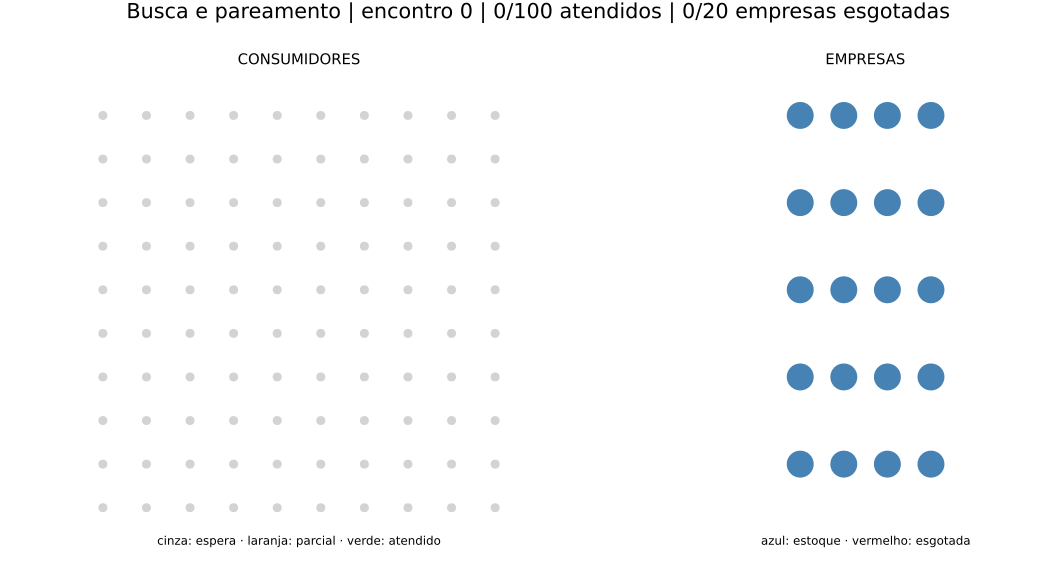
\includegraphics[width=0.95\textwidth,height=0.78\textheight,keepaspectratio]{assets/celula-50-quadro-000.png}
\end{frame}


\begin{frame}{4. Mercados com fricção  ("Search and Matching")}
\centering
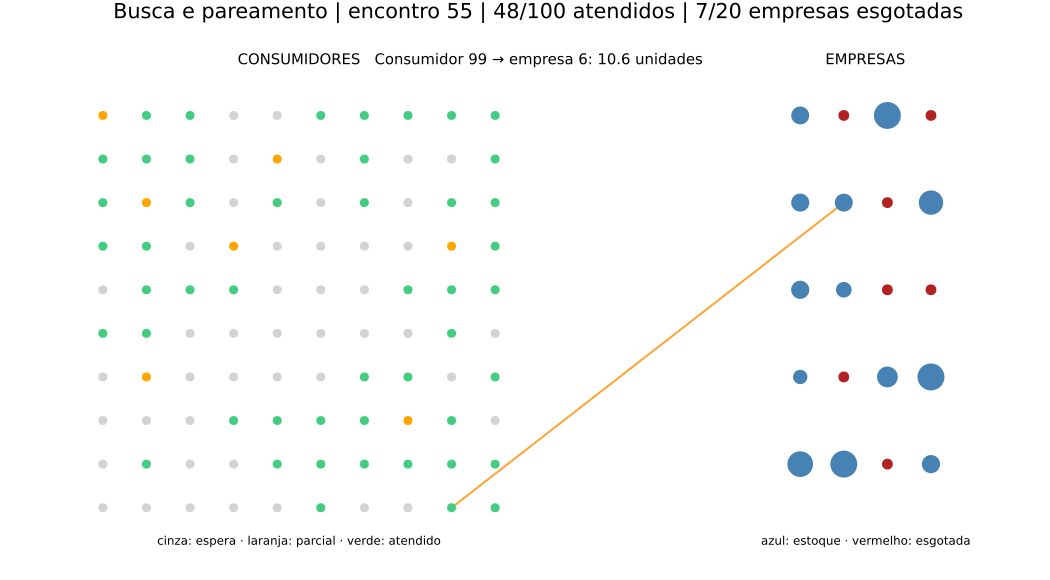
\includegraphics[width=0.95\textwidth,height=0.78\textheight,keepaspectratio]{assets/celula-50-quadro-055.png}
\end{frame}


\begin{frame}{4. Mercados com fricção  ("Search and Matching")}
\centering
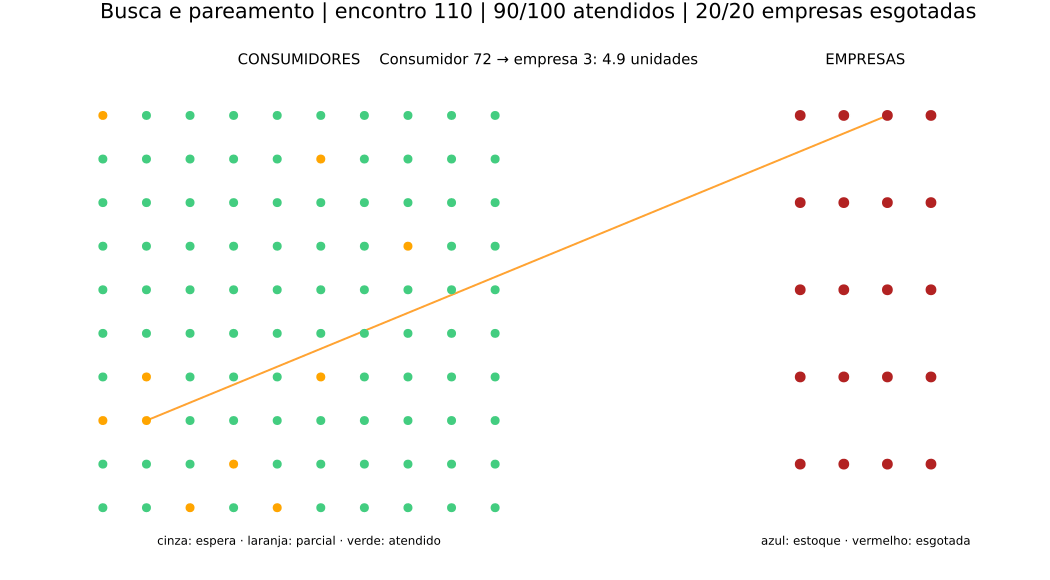
\includegraphics[width=0.95\textwidth,height=0.78\textheight,keepaspectratio]{assets/celula-50-quadro-110.png}
\end{frame}


\section{5. Revisão do ciclo completo}

\begin{frame}{5.1 Retomando o ciclo completo:}
\centering
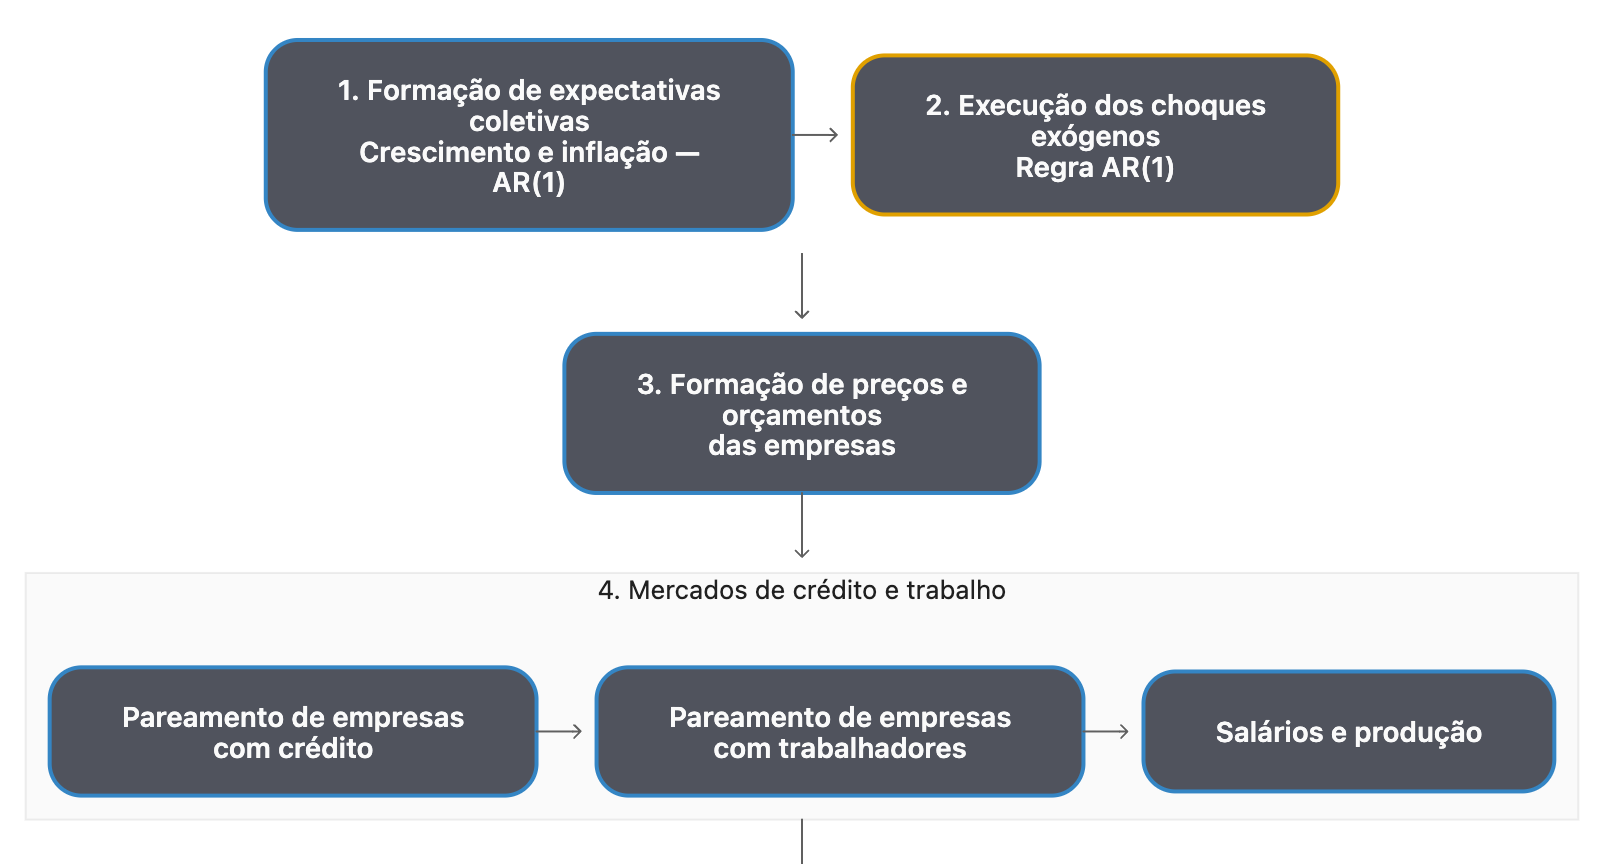
\includegraphics[width=0.95\textwidth,height=0.78\textheight,keepaspectratio]{assets/celula-53-novo-fluxo-completo-mermaid-diagram-parte-1.png}
\end{frame}


\begin{frame}{5.1 Retomando o ciclo completo:}
\centering
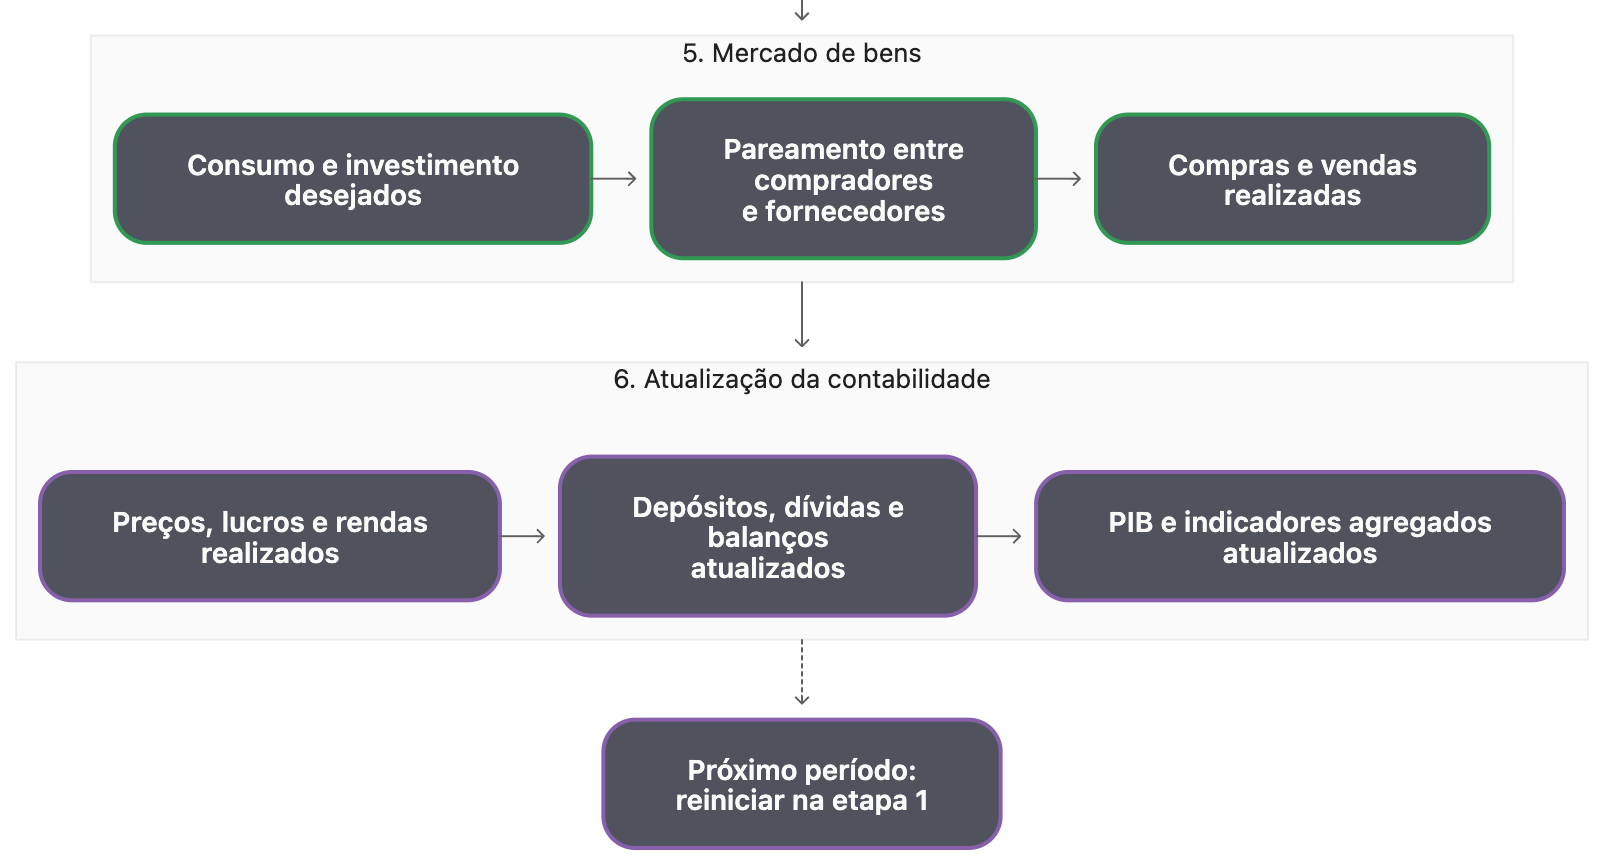
\includegraphics[width=0.95\textwidth,height=0.78\textheight,keepaspectratio]{assets/celula-53-novo-fluxo-completo-mermaid-diagram-parte-2.png}
\end{frame}


\begin{frame}{5.2 Resumo do Comportament dos Agentes}
\centering
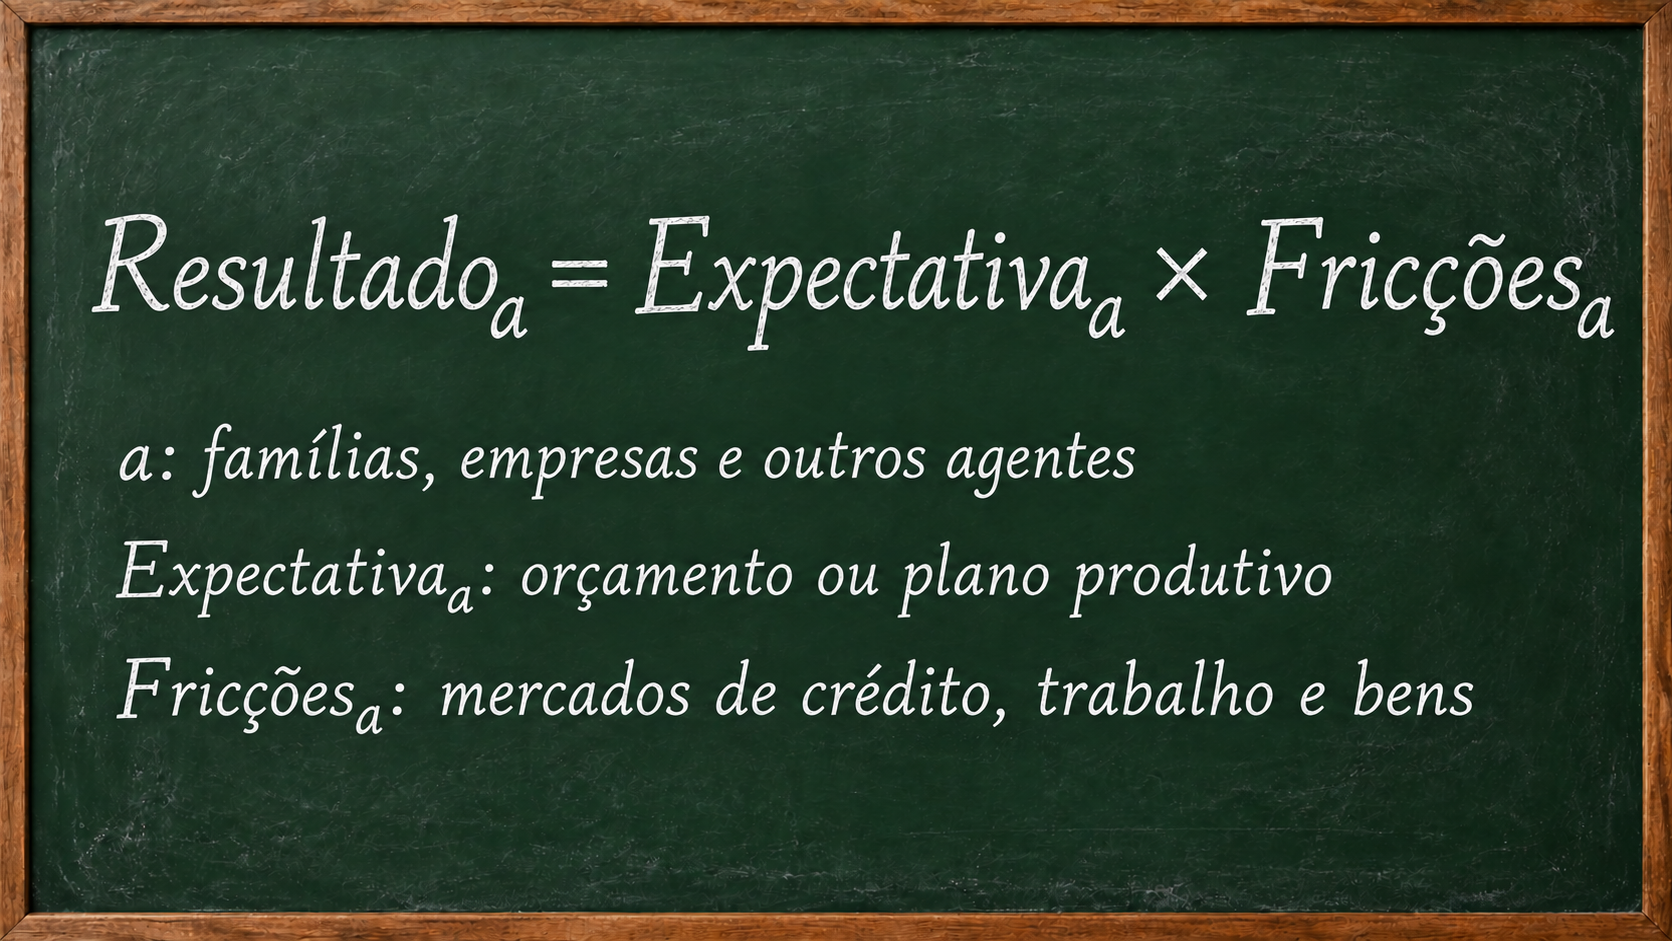
\includegraphics[width=0.95\textwidth,height=0.78\textheight,keepaspectratio]{assets/celula-55-image.png}
\end{frame}


\section{6. Resultados}

\begin{frame}[allowframebreaks]{6.1 Metodologia para mensuração de performance}
\normalsize
As previsões foram calculadas para dados fora da amostra de calibração e o erro do modelo foi comparado com os modelos abaixo.

Hipóteses nulas:

\begin{itemize}
\item
  AR (1): a própria regra autoregressiva que os agentes utilizam.
\item
  VAR (1): uma extensão com lags adicionais (\(z_{t-1},z_{t-2}...\)) do modelo AR (1).
\end{itemize}

Benchmarks:

\begin{itemize}
\item
  VECM (Vector Error Correction Model): O VECM é um modelo estatístico de séries temporais usado para analisar variáveis que possuem uma relação de equilíbrio de longo prazo, mesmo que sofram desvios temporários no curto prazo.
\item
  DSGE (Dynamic Stochastic General Equilibrium): Modelo DSGE Neo Keyneisiano padrão.
\end{itemize}

Foram feitas 500 simulações de Monte Carlo para o modelo e realizadas comparações com os dados realizados utilizando RMSE (root mean squared error) para as seguintes variáveis:

\begin{itemize}
\item
  PIB
\item
  Inflação
\item
  Consumo das famílias
\end{itemize}
\end{frame}


\begin{frame}[allowframebreaks]{6.1 Metodologia para mensuração de performance}
\normalsize
\begin{itemize}
\item
  Investimento
\item
  Euribor (``Taxa selic da Europa'')
\end{itemize}
\end{frame}


\begin{frame}[allowframebreaks]{6.2 Discussão dos resultados}
\normalsize
De maneira geral, o ABM \texttt{não\ apresentou\ melhoria\ significativa} em relação aos benchmarks. Apesar disso, para algumas variáveis houve uma melhoria expressiva mas sem significância.

Mesmo não havendo uma melhoria relevante, é interessante notar que, tendo em vista o que foi apresentado sobre verossimilhança e escala do modelo, o ABM permite realizar uma quantidade bem maior de previsões e, portanto, pode ser considerado mais rico (vide meso-level discutido por Brian Arthur).

Abaixo temos uma das tabelas de resultados do trabalho.
\end{frame}


\begin{frame}{6.2 Discussão dos resultados}
\centering
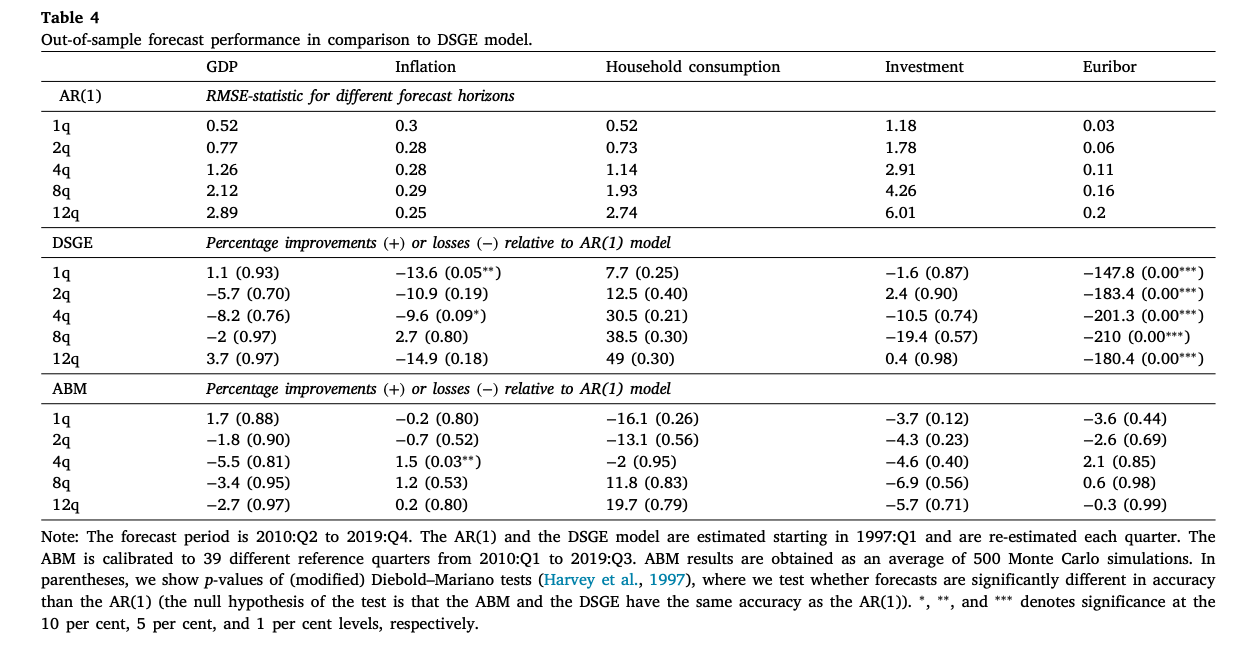
\includegraphics[width=0.95\textwidth,height=0.78\textheight,keepaspectratio]{assets/Screenshot 2026-10-02 at 17.46.06.png}
\end{frame}


\section{7. Observações críticas}

\begin{frame}[allowframebreaks]{7. Observações críticas}
\normalsize
De maneira geral, o modelo é bem construído e parcialmente bem-sucedido ao realizar previsões similares aos modelos padrões da economia mainstream (DSGE).

Constitui uma tentativa inicial de mover os ABMs macroeconômicos do território dos \texttt{fatos\ estilizados}, ou seja, da reprodução qualitativa de regularidades empíricas, para o campo \texttt{quantitativo}. Os resultados no entanto foram bastante limitados, ainda mais tendo em vista a complicação do modelo.

Assim, podemos apontar algumas fragilidades do modelo que podem ser objeto de futuras melhorias:

\begin{itemize}
\item
  Sistema bancário com um banco representativo.
\item
  A grande parte dos parâmetros fixos estão `atrasados' em relação ao tempo de previsão e não levam em conta alterações estruturais.
\end{itemize}
\end{frame}


\begin{frame}[allowframebreaks]{7. Observações críticas}
\normalsize
\begin{itemize}
\tightlist
\item
  É possível argumentar que o modelo é ``autorrealizável'' ao colocar nos agentes expectativas que equivalem ao aprendizado de uma série histórica inteira.
\end{itemize}
\end{frame}


\section{8. Referências}

\begin{frame}[allowframebreaks]{8. Referências}
\normalsize
DAWID, Herbert; DELLI GATTI, Domenico. \href{https://papers.ssrn.com/sol3/papers.cfm?abstract_id=3112074}{Agent-Based Macroeconomics}. \emph{Bielefeld Working Papers in Economics and Management}, n.~02-2018, 2018. DOI: \href{https://doi.org/10.2139/ssrn.3112074}{10.2139/ssrn.3112074}.

GLIELMO, Aldo; DEVETAK, Mitja; MELIGRANA, Adriano; POLEDNA, Sebastian. \href{https://arxiv.org/abs/2502.13267}{BeforeIT.jl: High-Performance Agent-Based Macroeconomics Made Easy}. \emph{arXiv}, arXiv:2502.13267, 2025. DOI: \href{https://doi.org/10.48550/arXiv.2502.13267}{10.48550/arXiv.2502.13267}.

HOMMES, Cars; ZHU, Mei. \href{https://doi.org/10.1016/j.jet.2013.09.002}{Behavioral Learning Equilibria}. \emph{Journal of Economic Theory}, v. 150, p.~778--814, mar. 2014. DOI: \href{https://doi.org/10.1016/j.jet.2013.09.002}{10.1016/j.jet.2013.09.002}.
\end{frame}


\begin{frame}[allowframebreaks]{8. Referências}
\normalsize
LEONTIEF, Wassily W. \href{https://www.scientificamerican.com/article/input-output-economics/}{Input-Output Economics} (A economia do insumo-produto). \emph{Scientific American}, v. 185, n.~4, p.~15--21, 1951. DOI: \href{https://doi.org/10.1038/scientificamerican1051-15}{10.1038/scientificamerican1051-15}.

POLEDNA, Sebastian; MIESS, Michael Gregor; HOMMES, Cars; RABITSCH, Katrin. \href{https://www.sciencedirect.com/science/article/pii/S0014292122001891}{Economic forecasting with an agent-based model}. \emph{European Economic Review}, v. 151, art. 104306, 2023. DOI: \href{https://doi.org/10.1016/j.euroecorev.2022.104306}{10.1016/j.euroecorev.2022.104306}.
\end{frame}


\section{Anexos}

\begin{frame}[allowframebreaks]{A1: Observações}
\normalsize
\begin{itemize}
\item
  Uma unidade monetária do modelo equivale a um milhão de euros.
\item
  Empresas estrangeiras fazem parte do vetor de produtos no search and matching
\end{itemize}
\end{frame}


\begin{frame}[allowframebreaks]{A2: ODD+D - resumo sintético do BeforeIT}
\normalsize
Seguindo a divisão em \textbf{Visão geral, Conceitos de projeto e Detalhes} do \href{https://github.com/danielbandrade/odd-d-abm-extractor/blob/main/references/odd-d-protocol.md}{protocolo ODD+D indicado}:
\end{frame}


\begin{frame}[allowframebreaks]{I. Visão geral}
\normalsize
\textbf{Propósito e agentes --- explícito.} O modelo simula a economia austríaca para produzir previsões macroeconômicas e analisar cenários. Representa famílias, empresas, governo, banco comercial, banco central e resto do mundo. A calibração usada no seminário contém 8.873 pessoas, 624 empresas, 156 entidades públicas e 312 consumidores externos, distribuídos por 62 setores. Cada passo da simulação equivale a um trimestre. O estudo original propõe escala 1:1; a execução apresentada no seminário usa escala reduzida.

\textbf{Sequência --- explícito.} Em cada trimestre, formam-se expectativas; empresas planejam produção, preços e contratações; ocorrem os mercados de crédito, trabalho e bens; por fim, a contabilidade e os indicadores agregados são atualizados.
\end{frame}


\begin{frame}[allowframebreaks]{II. Conceitos de projeto}
\normalsize
\textbf{Decisões, aprendizado e interação --- explícito.} Os agentes seguem regras comportamentais simples sob incerteza. Empresas ajustam suas decisões às vendas anteriores e às expectativas de crescimento e inflação; famílias ajustam gastos à renda. Os parâmetros das expectativas AR(1) são reestimados com os dados observados. As trocas acontecem por \emph{search and matching}, de forma descentralizada e probabilística, e a matriz insumo-produto conecta os setores.

\textbf{Emergência --- explícito.} PIB, inflação, desemprego, estoques e oscilações econômicas resultam das decisões e transações, sem que seus valores sejam impostos ao sistema. Choques externos também afetam esses resultados; por isso, não se deve classificar todo movimento observado como endógeno.
\end{frame}


\begin{frame}[allowframebreaks]{III. Detalhes}
\normalsize
\textbf{Inicialização e observação --- explícito.} Censo, demografia empresarial, contas nacionais e matriz insumo-produto fundamentam a calibração. O modelo registra resultados agregados e setoriais; previsões são obtidas por múltiplas simulações com diferentes choques e encontros nos mercados.

\textbf{Limite da descrição --- não relatado integralmente no artigo.} Parte das equações comportamentais, dos algoritmos de mercado e dos procedimentos de calibração é remetida aos apêndices. O artigo também não descreve aprendizado coletivo por imitação ou uma rede social de comunicação entre agentes. \href{/Users/danielbandrade/Documents/programing/BeforeIT-dba/dba-studies/model-mechanics/odd-d-description.md}{Descrição ODD+D detalhada do modelo}.
\end{frame}


\begin{frame}[allowframebreaks]{A3: Varredura de complexidade do BeforeIT}
\normalsize
O problema em estudo é a \textbf{previsão da economia austríaca} por meio de uma modelagem baseada em agentes. Em vez de determinar previamente o PIB, a inflação e o desemprego, o modelo simula as decisões e transações dos agentes; essas variáveis são calculadas a partir dos resultados de cada trimestre.
\end{frame}


\begin{frame}[allowframebreaks]{A3: Varredura de complexidade do BeforeIT}
\normalsize
\textbf{a) Tipos e quantidades de agentes.} Na calibração utilizada no seminário, há 8.873 pessoas: 4.118 trabalhadores ativos, 4.130 pessoas inativas, 624 proprietários de empresas e um proprietário do banco. Há também 624 empresas, um banco comercial representativo, um banco central e um governo. O governo representa a demanda de 156 entidades públicas; o resto do mundo representa 312 consumidores externos e a oferta de importações em 62 setores. Os proprietários já estão incluídos nas 8.873 pessoas, portanto não devem ser somados novamente às empresas. Esses números pertencem à \textbf{simulação em escala reduzida} usada no notebook; o trabalho original também propõe uma representação em escala 1:1.
\end{frame}


\begin{frame}[allowframebreaks]{A3: Varredura de complexidade do BeforeIT}
\normalsize
\textbf{b) Interação entre os agentes.} As empresas procuram crédito, contratam trabalhadores, compram insumos e vendem bens. As pessoas recebem salários, rendimentos ou benefícios e decidem quanto consumir e investir. O governo arrecada impostos, realiza transferências e compra bens. O banco concede empréstimos, enquanto o banco central define a taxa básica de juros. O resto do mundo participa por meio de importações e exportações. Cada compra, venda ou pagamento atualiza a contabilidade dos agentes envolvidos.
\end{frame}


\begin{frame}[allowframebreaks]{A3: Varredura de complexidade do BeforeIT}
\normalsize
\textbf{c) Conexão entre os agentes.} As conexões se formam principalmente nos mercados de crédito, trabalho e bens, por mecanismos de \emph{search and matching}. Os compradores e vendedores são associados de maneira descentralizada e probabilística. Entre empresas, a matriz insumo-produto estabelece quais setores fornecem os insumos necessários à produção de outros setores. Assim, uma mudança na atividade de uma empresa pode alcançar outras empresas, seus trabalhadores e consumidores.
\end{frame}


\begin{frame}[allowframebreaks]{A3: Varredura de complexidade do BeforeIT}
\normalsize
\textbf{d) Adaptação, aprendizado e evolução.} A cada trimestre, os agentes ajustam suas decisões às condições observadas: empresas alteram produção desejada, preços, contratações e demanda por crédito; famílias ajustam seus gastos à renda e aos preços. As expectativas coletivas de crescimento do PIB e inflação seguem regras AR(1), cujos parâmetros são reestimados com os dados acumulados. Esse é o principal mecanismo de \textbf{aprendizado} do modelo. As regras comportamentais em si permanecem definidas; não há, nesta implementação, evolução de novas estratégias por seleção ou imitação.
\end{frame}


\begin{frame}[allowframebreaks]{O modelo como sistema complexo}
\normalsize
\textbf{e) Padrões e comportamentos emergentes.} PIB, inflação, desemprego, estoques e oscilações da atividade econômica resultam da agregação das decisões e transações. Por exemplo, uma empresa que vende menos do que esperava pode acumular estoques, reduzir a produção e contratar menos no trimestre seguinte. A queda de renda dos trabalhadores pode então diminuir a demanda de outras empresas.
\end{frame}


\begin{frame}[allowframebreaks]{O modelo como sistema complexo}
\normalsize
\textbf{f) Mecanismos de emergência e auto-organização.} Esses resultados surgem dos ajustes sucessivos das expectativas e dos encontros nos mercados com fricção. Nenhum agente determina sozinho o nível final de produção ou emprego, e não há um mecanismo central que faça todos os mercados se equilibrarem a cada trimestre. Nesse sentido, há \textbf{auto-organização das transações e dos resultados macroeconômicos}. Isso não significa ausência de instituições centrais: governo e banco central exercem, respectivamente, funções fiscais e monetárias.
\end{frame}


\begin{frame}[allowframebreaks]{O modelo como sistema complexo}
\normalsize
\textbf{g) Papel da cooperação.} A cooperação aparece como \textbf{interdependência econômica}: empresas dependem de fornecedores, trabalhadores, crédito e compradores para produzir e vender; famílias dependem de renda para consumir. Essas relações permitem o funcionamento conjunto da economia, embora os agentes não busquem um objetivo coletivo nem adotem uma estratégia explícita de cooperação.
\end{frame}


\end{document}
